\documentclass[10pt,conference,compsocconf]{IEEEtran}

\usepackage{hyperref}
\usepackage{graphicx}	% For figure environment


\begin{document}
\title{Higgs Boson: a Machine Learning Challenge}

\author{
  Timothée Duran, Marijn van der Meer, Bradley ?? 
}

\maketitle

\begin{abstract}

 This report explain the attempts we made for our participation in the Higgs boson machine learning challenge. This was a part of the Machine Learning course taught at EPFL. The goal was to find out through the given data from CERN if there are Higgs boson in the observations. We built different models that we optimized. This paper presents our results. 
\end{abstract}

\section{Introduction}\label{sec: introduction}
The Higgs boson, generated by quantum excitation of the Higgs field, is an elementary particle discovered at CERN in 2013. Rarely, a collision between protons generates a Higgs boson that then decays rapidly. The decay does, however, leave a signature that can be measured. In this project, the decay signatures, which come from ATLAS experiment~\cite{Aad_2012} and the CMS experiment~\cite{Chatrchyan_2012} that led to the discovery of this particle, were introduced into machine learning models in order to find a accurate binary classifier. The objective was to develop a model that would allow the identification of the Higgs boson signatures from background noise.
\section{Models and Methods}\label{sec: models_methods}
Describe your idea and how it was implemented to solve
  the problem. Survey the related work, giving credit where credit is
  due.
  \subsection{Pre-processing and feature generation}\label{subsec:pre-proc}
  The data provided was a training set of 250'000 events of 30 features and a test set of around 568'238 events. Features varied from floating points to integer values and labels provided were -1 for background and 1 for boson. Those labels were changed to 1 for boson and 0 for background for computational reasons with logistic regression. Invalid data are marked with the value \textit{-999} and have to be removed. To do this, we have two choices, either we remove the complete sample, or we replace the given value with the mean or median value of the feature. However, since a significant number of invalid values are present, we choose the second method to keep as many samples as possible. The data being normalized after this cleaning, replacing the value by this mean is equivalent to giving it no value. Throughout testing, we noticed that using the median over the mean reduces the error. For outfitting values, we plotted the data into histograms to evaluate how and whether other out-layers should be processed. We then choose to apply the same technique as above for all values that are outside a defined range. \textbf{TODO Explain range}. An example of histogram of data before and after the processing can be found at figure \ref{fig:processing_compare}.
    After invalid values and outfitters were replaced by the medians of our features, we engineered our features by adding a bias column and a polynomial expansion $\phi:[X]\rightarrow [1, X, X^2,...,X^k]$ where $X\in \mathbb{R}^{N30}$. The data was then further standardised using Z-score standardisation, e.g. $Z = \frac{X - \mu}{\sigma}$.
    
  \subsection{
  Model implementation
  }
  To fit our data, we implemented six different models: 
    \begin{itemize}
        \item Linear regression using normal equations, gradient descent and stochastic gradient descent 
        \item Ridge regression using normal equations
        \item Logistic regression using gradient descent 
    \end{itemize}
    These different models were evaluated based on their loss and accuracy on validation sets created from a $80\%:20\%$ 5-fold cross-validation. Evaluating all models over 100 epochs with the same learning rate of 0.01, regularisation parameter of 0.02 and polynomial expansion of degree 2, we observed that (regularised) logistic regression performed much better than the others, c.f. Table~\ref{tab:basic_training}. Thus, rather than tuning all of the models in order to improve their scores, we chose to concentrate on regularised logistic regression as it seemed the most promising from the start. 
    
    \subsection{Hyperparameter tuning}\label{subsubsec: parameter_tuning}
    To tune the hyperparameters of our (regularised) logistic regression model, we performed a randomised grid search~\cite{jonasbenner2019}. The aim of randomized grid search is to pick $k$ random combinations from a grid of possible. We chose this approach compared to a classical grid search in order to reduce the computational and thus also the time price. The performance of parameters was again evaluated using 5-fold cross-validation. The combination resulting in minimal loss were kept. This was used to choose the best learning rate from  $[0.03,0.3]$, regularization parameter $[0.001,0.1]$ and the degree of polynomial expansion $[1,7]$.
    
\section{Results}\label{sec: results}
Following hyperparameter tuning (c.f. \ref{subsubsec: parameter_tuning}), regularized logistic regression 
\section{Discussion}\label{sec: discussion}
Discuss the strengths and weaknesses of your
  approach, based on the results. Point out the implications of your
  novel idea on the application concerned.
\section{Summary}\label{sec: summary}
Summarize your contributions in light of the new
  results.
The aim of a scientific paper is to convey the idea or discovery of
the researcher to the minds of the readers. The associated software
package provides the relevant details, which are often only briefly
explained in the paper, such that the research can be reproduced.
To write good papers, identify your key idea, make your contributions
explicit, and use examples and illustrations to describe the problems
and solutions.

\subsection{Figures and Tables}
\begin{table}[htbp]
  \centering
  \begin{tabular}[c]{|l||l|l|l|}
    \hline
    &Average loss&Average accuracy \\
    \hline
    Least squares GD & 0.18 & 50.16\% \\
    Least squares SGD & 0.29 & 50.90\%\\
    Least squares Normal & 0.15 & 42.68\%\\
    Ridge regression Normal & 0.15 & 42.68\%\\
    Logistic regression GD & 0.58 & 73.24\%\\
    Regularized logistic regression GD & 0.58 & 73.24\% \\
    \hline
  \end{tabular}
  \caption{Accuracy and loss on 20\% validation set for 100 epochs, learning rate of 0.01 and regularization of 0.02. }
  \label{tab:basic_training}
\end{table}
\begin{figure}[tbp]
  \centering
  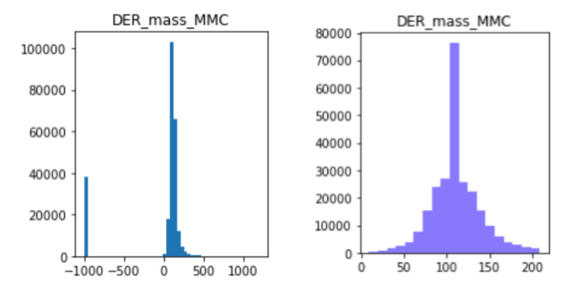
\includegraphics[width=\columnwidth]{processing_compare}
  \caption{Histogram DER\_mass\_MMC values before and after preprocessing.}
  \vspace{-3mm}
  \label{fig:processing_compare}
\end{figure}

Use examples and illustrations to clarify ideas and results. For
example, by comparing Figure~\ref{fig:denoise-fourier} and
Figure~\ref{fig:denoise-wavelet}, we can see the two different
situations where Fourier and wavelet basis perform well. 





\bibliographystyle{IEEEtran}
\bibliography{literature}

\end{document}
